\documentclass[a4paper,11pt,oneside]{article}
\usepackage[headheight=28pt,margin=3cm]{geometry}
\usepackage[utf8]{inputenc}
\usepackage[T1]{fontenc}
\usepackage[english]{babel}
\usepackage[ddmmyy]{datetime}
\usepackage{titlesec}
\usepackage{tikz}
\usetikzlibrary{arrows}
\usepackage{color}
\usepackage{float}
\usepackage{fancyvrb}
\usepackage[normalem]{ulem}

\usepackage{forest}

\usepackage{fancyhdr}

\usepackage{pdfpages}
\usepackage{amssymb}
\usepackage{amsmath}
\usepackage{listings}
\usepackage{comment}
\usepackage{hyperref}
\usepackage[all]{hypcap}
\usepackage{caption}
\usepackage{xcolor}
\hypersetup{
	colorlinks   = true, %Colours links instead of ugly boxes
	urlcolor     = blue, %Colour for external hyperlinks
	linkcolor    = black, %Colour of internal links
	citecolor    = black %Colour of citations
}
\usepackage{multirow}
\usepackage{cleveref}
\usepackage{xspace}
\usepackage{array}
\usepackage{makecell}

\renewcommand\theadalign{bc}
\renewcommand\theadfont{\bfseries}
\renewcommand\theadgape{\Gape[4pt]}
\renewcommand\cellgape{\Gape[4pt]}

\renewcommand{\choose}[2]{\ensuremath{
\scriptsize
\begin{pmatrix}
#1\\
#2
\end{pmatrix}}}
\renewcommand{\vec}[1]{\ensuremath{\mathbf #1}}
\newcommand{\set}[1]{\ensuremath{\left\{#1\right\}}}
\newcommand{\pr}[1]{\ensuremath{Pr\left\{#1\right\}}}
\newcommand{\ex}[1]{\ensuremath{\mathds{E}\left[#1\right]}}
\newcommand{\vari}[1]{\ensuremath{V\left(#1\right)}}
\newcommand{\todo}{\textcolor{red}{\huge{\textbf{TODO}}}}
\newcommand{\abs}[1]{\ensuremath{\left|#1\right|}}
\newcommand{\swarco}{\textsc{swarco}}
\newcommand{\mycal}[1]{\ensuremath{\mathcal{#1}}}
\newcommand{\Ex}[1]{\ensuremath{\mathbb{E}\left[#1\right]}}

\usepackage{mathtools}
\DeclarePairedDelimiter\ceil{\lceil}{\rceil}
\DeclarePairedDelimiter\floor{\lfloor}{\rfloor}
\usepackage{etoolbox}
%\AtBeginEnvironment{align}{\setcounter{equation}{0}}


\usepackage[square, numbers, comma, sort&compress]{natbib}  % Use the "Natbib" style for the references in the Bibliography
\bibliographystyle{unsrtnat}
\setcitestyle{number, open={[},close={]}}
\usepackage{verbatim}  % Needed for the "comment" environment to make LaTeX comments

\usepackage{import}


\usepackage{subcaption} % Only use one of the two
% \usepackage{subfig}    % Only use one of the two

\usepackage{graphicx}
\usepackage{svg}
\DeclareGraphicsExtensions{.svg}
\svgpath{{../include/}} 
\definecolor{dkgreen}{rgb}{0,0.45,0}
\definecolor{gray}{rgb}{0.5,0.5,0.5}
\definecolor{mauve}{rgb}{0.30,0,0.30}
\usepackage{notation} % Notation styles from Sutton & Barto book

%%%% TODO: Change this if needed! %%%%
\newcommand{\implementationlanguage}{python}

\newcommand{\tnode}{\textit{node}\xspace}
\newcommand{\replace}[1]{\textcolor{red}{\huge{\textbf{#1}}}}
\setlength\parindent{0pt}
\setlength\parskip{0.5em}


\lstset{frame=tb,
	language=\implementationlanguage,
	aboveskip=3mm,
	belowskip=3mm,
	showstringspaces=false,
	columns=flexible,
	basicstyle={\small\ttfamily},
	numbers=left,
	numberstyle=\footnotesize,
	keywordstyle=\color{dkgreen}\bfseries,
	commentstyle=\color{red},
	stringstyle=\color{mauve},
	frame=single,
	breaklines=true,
	breakatwhitespace=false
	tabsize=1
}


\title{Traffic Light Control by Reinforcement Learning\\\rule{10cm}{0.5mm}}
\author{Henrik Sejer Pedersen
  \\
  Supervisor: Marco Chiarandini\\
  \rule{5.5cm}{0.5mm}
}
\date{\longdate\today}



\begin{document}
\maketitle
\vfill
\clearpage
\pagestyle{fancy}
\lhead{\emph{Table of Contents}}
\rhead{}
\tableofcontents
\clearpage

%%%%%%%%%%%%%%
% Chapters
%%%%%%%%%%%%%%



\pagestyle{fancy}
\lhead{\emph{Introduction}}
% !TeX root = ../report.tex
\paragraph{Abstract}

% !TeX root = ../report.tex
\section{Introduction}

With a steady increase in urbanization on top of already existing traffic problems in urban areas, the need for improving the traffic flow becomes ever more apparent. 
In urban areas, it is likely to be very costly if at all feasible to tear up existing infrastructure to accommodate better roads, so we turn our focus to the dynamic element present in most urban areas today, traffic lights.

Traffic lights provide an opportunity to influence the traffic flow in urban areas utilizing software, be it simple fixed-time, scheduled light changes or sophisticated traffic-reactive systems. 

In this project, we look into the online, adaptive optimization strategies through reinforcement learning. Some of the early adaptive approaches SCAT\cite{SCAT1980} which was implemented in Sydney around 1980 and SCOOT\cite{SCOOT1991}, which is in extensive use to this date, focus on the coordination of multiple intersections, often known as \emph{urban traffic control}. 
In \citet{SCOOT1991}, the coordination serves to shift traffic light cycles such that average queue lengths and vehicle stops are minimized, but still rely on the individual traffic light cycle to be efficient.

\vspace*{1em}

In this project, we seek to explore the application of reinforcement learning to control the individual traffic light, using only existing infrastructure.

At a very high level, reinforcement learning consist of an \textit{agent} placed into some \textit{envrionment}, where it takes actions and receive some \textit{reward} based on those actions. Over time, the goal of the agent is to learn which actions to take in what situations to maximize the expected future reward. We will only cover a small part of reinforcement learning in this project, for a wider overview refer to \citet{RLBook2018}.

The application of reinforcement learning to the field of traffic light control has been examined many a time\citep{Thorpe96trafficlight}\citep{wiering2000multi}\citep{AbdulhaiPringleKarakoulas}\citep{ItamarEtAl}\citep{bakker2010traffic}\citep{ExploringRewardDefinitions}\citep{ModelsAndAlgorithms}\citep{StateRepresentations}.
However, due to the data made available by swarco Danmark A/S, we can  provide further insight into the details of applying reinforcement learning to traffic light control based on existing infrastructure and information.

\citet{Thorpe96trafficlight} showed great potential of reinforcement learning applied to traffic light control with their implementation of the SARSA algorithm on three different complete-knowledge state representations on a grid of 4x4 intersections, approaching the performance of an optimal policy.

\citet{wiering2000multi} presented three different state representations for the multi-agent problem, where varying degrees of global information was included in the states. 
He found that more global information did not necessarily mean better performance, but some global information did perform better than none.

\citet{AbdulhaiPringleKarakoulas} implemented Q-learning which is a temporal-difference algorithm, on a single-agent basis, with comments on ideas to improve it for multi-agent use. 
They used state information which could be estimated from detector data, in the form of queue lengths and elapsed phase time.  
The reward used is a penalty in the form of total vehicle delay between decision points. 
Additionally, they made use of a neural-network-like structure (CMAC) to approximate the value function, which provided some generalization and should, to some extent, improve behavior in unobserved states.

\citet{ItamarEtAl} used an actual neural network for value function approximation, which should perform even better in unobserved states compared to the CMAC. The state used is also significantly improved, as it incorporates only what they refer to as \emph{relative traffic flow}, calculated for every upstream lane as traffic flow in that lane divided by average traffic flow of all upstream lanes of the intersection. Such a state representation can be implemented using detector data only. The reward is based on average delay, giving a negative reward if an action increases the average delay, but a positive reward if it is decreased.





%\clearpage
\pagestyle{fancy}
\lhead{\emph{Instance Definition}}
% !TeX root = ../report.tex
\section{Instance definition}
In this section, we introduce a traffic light located in southern Odense, Denmark and its implementation in the microscopic traffic simulator SUMO -- \textit{Simulation of Urban MObility}.

\subsection{Network topology}
The company \swarco{} provided the data and network information we use in this project. We look at a traffic light controlled intersection located in southern Odense, Denmark, depicted in \cref{appendix:techdrawloop}. We modeled the intersection in the microscopic traffic simulator SUMO, without the inclusion of bicycles, as the available data on bicycles is quite limited.

\subsubsection{Induction Loops}
In the network, a number of vehicle detectors are present, in the form of \textit{induction loops}.
In \cref{appendix:techdrawloop}, the locations of induction loops relevant to the intersection is visualized. \Cref{fig:inductionsignatures} describes the meaning of the visualization.

\begin{figure}[!htb]
  \centering
  \includeinkscape[scale=3]{signaturer}
  \caption{Induction loop signatures}
  \label{fig:inductionsignatures}
\end{figure}

The induction loops in the intersection cover vehicles quite well, but are quite lacking when it comes to bicycles, for this reason, bicycles are excluded from the project.


\subsubsection{Traffic light movements}
\Cref{appendix:techdrawmovement} visualizes the traffic signal groups in the intersection. \Cref{tab:intersectionmovements} describes the traffic signal strings on the drawing. A single signal can control multiple of these movements, denoted by, for instance, A1$+$A1v denotes a single signal controlling both left-turn and straight movements of A1.

\begin{table}[!htb]
  \centering
  \begin{tabular}{|c|c|}\hline
      string & meaning \\\hline
       A/B/C/\ldots\# & Upstream movement following road\\\hline
       A\#Cy & Straight-ahead bicycle movement from A\#\\\hline
       A\#v & Left-turn movement from A\#\\\hline
       A\#h & right-turn movement from A\#\\\hline
  \end{tabular}
  \caption{Explanation of traffic light movement strings for \cref{appendix:techdrawmovement}\\\replace{todo: better string representation}}
  \label{tab:intersectionmovements}
\end{table}

\subsection{SUMO Introduction}
SUMO, short for \textit{Simulation of Urban MObility}, is a microscopic, well-established general-purpose traffic simulator. It has been around since 2001 and is an open source project. What makes it particularly interesting for this project, is the ability to control elements of the simulation externally, through a well-defined API. With this API, gathering information from the simulation for our agent is made simple, while also providing a way for our agent to control each traffic light.

\subsection{Implementing the intersection in SUMO}
SUMO uses a directed graph representation to define a traffic network, with some extra information. 
\textit{Nodes} in the graph are points connected by one or more \textit{edges}. Nodes contain connection data, which is (potentially) a many-to-many mapping of incoming lanes to outgoing lanes. The edges carry the lane information, allowing any number of adjacent lanes (within computational reason) to follow any single edge between two nodes. As such, each edge defines a set of up- or down-stream lanes, possibly consisting of multiple traffic movements.


\begin{figure}[!htb]
  \centering
  \includeinkscape[scale=0.2]{sumo}
  \caption{Intersection as implemented in SUMO, visualised by SUMO-GUI\\\replace{todo: better image}}
  \label{fig:sumointerimpl}
\end{figure}

The primary discrepancies between the actual intersection and the one implemented in SUMO are the missing induction loop D18. The induction loop is not present in the SUMO implementation as SUMO only allows placing induction loops on lanes.

\subsection{Vehicle data}

Along with technical drawings of the intersection, files describing the traffic flow exist in the form of 5 minutes aggregated readings from the 25 induction loops present in the intersection.
To use this data in a meaningful way, we define orderings of the induction loops, each of which defines a route in the network. 

Populating these sets with the input data can be modeled as an integer linear programming problem, and draws many parallels with the generalized set covering problem.
Unfortunately, the induction loop readings have proven non-perfect, so we propose two different models.

The first model assumes that the induction loops never miss any vehicles, but may overcount.
The second model assumes that the induction loops do not overcount, but may miss vehicles. 

Both models give a vehicle count for each route for a single 5-minute interval and are called once for each such period.
Solving for shorter intervals increase the network load in the simulation, we use the second model in this project.

\subsubsection{Overcounts, no misses}
Given a set of routes $R$, a set of detectors $D$, a binary route representation as defined below by $B_{ij}$, and upper bounds for \textit{total} number of vehicles passing a detector, defined below by $C_i$. 
Select the number of vehicles to follow each route, such that the number of vehicles passing each detector is maximized for all detectors, given the single constraint:
\begin{itemize}
  \item No more than $C_i$ vehicles can pass detector $D_i$, $\forall i \in \set{1, 2, \ldots, |D|}$
\end{itemize}

For convenience we define the sets $I = \set{1, 2, \ldots, |D|}$, and $J = \set{1, 2, \ldots, |R|}$.

Let $B{ij}$ be a binary constant such that:
\[
  B_{ij} = \begin{cases}
    1 & \text{if route j passes detector i}\\
    0 & \text{otherwise}
  \end{cases}\quad \forall i \in I, j \in J
\]
Let $C_i$ be an an detected number of vehicles at detector $D_i,\ \forall i \in I$
Let $x_j$ be an integer variable with a lower bound of 0, indicating the number of vehicles following route $j, \forall j \ in J$
\begin{align*}
  \begin{array}{rrcll}
    \text{Maximize} & \displaystyle\sum_{j\in J}x_j \cdot \sum_{i\in I}B_{ij}&&&\\
    \text{s.t.} & \displaystyle\sum_{j\in J}B_{ij}\cdot x_j & \leq & C_i & \qquad \forall i \in I\\
    & x_j & \in & \mathbb{N}&\qquad \forall j \in J\\
    & x_j & \geq & 0&\qquad \forall j \in J
  \end{array}
\end{align*}
The objective function maximizes the total sum of vehicles passing detectors. The outer sum sums over each route, and the second sum computes the number of detectors in the route from the outer sum.

The first constraint ensures that the sum of vehicles passing a detector does not surpass its capacity.

The second constraint ensures that the number of vehicles entering the simulation is integer.

The Third constraint ensures that the number of cars on each route must be non-negative.

\subsubsection{Misses, no overcounts}
The previous model can with a few changes be modified, such that the vehicle counts act as lower bounds rather than upper bounds.
Treating vehicle counts as lower bounds will put a more significant strain on the network, as more vehicles enter the simulation, which is desired.

\begin{align*}
  \begin{array}{rrcll}
    \text{Minimize} & \displaystyle\sum_{j\in J}x_j \cdot \sum_{i\in I}B_{ij}&&&\\
    \text{s.t.} & \displaystyle\sum_{j\in J}B_{ij}\cdot x_j & \geq & C_i & \qquad \forall i \in I\\
    & x_j & \in & \mathbb{N}&\qquad \forall j \in J\\
    & x_j & \geq & 0&\qquad \forall j \in J
  \end{array}
\end{align*}

The objective of the new model is to minimize the number of vehicles passing induction loops, while enforcing that at least the observed number of vehicles pass.

It is important to note that in this model, $B_{i\cdot}$ must contain at least $one$ $1$ to be feasible for all $i$, whereas this was not the case for the previous model.

%\clearpage
\pagestyle{fancy}
\lhead{\emph{Introduction to reinforcement learning}}
% !TeX root = ../report.tex
\section{Introduction to reinforcement learning}
Reinforcement learning is a machine learning paradigm dedicated to solving sequential decision processes. The definition of a reinforcement learning algorithm given by \citet[chap. 3]{RLBook2018}, is an algorithm which can solve a specific kind of sequential decision problem, namely those which can be described formally by a \textit{finite Markov decision process}.


\subsection{Finite Markov Decision Processes}

The Markov decision process provides a formal description of sequential decision problems. 

In this project, we define a Markov decision process by a 4-tuple $(\mathcal{S},\mathcal{A},\mathcal{R}, p)$, where $\mathcal{S}$ is the finite state-space, $\mathcal{A}$ is the finite action-space, $\mathcal{R} \subset \mathbb{R}$ is the finite reward-space, and the dynamics function $p : \mathcal{S} \times \mathcal{R} \times \mathcal{S} \times \mathcal{A} \rightarrow [0,1]$, defined in \cref{eq:p_def}, describes the conditional probability of entering a state $s' \in \mathcal{S}$ with reward $r \in \mathcal{R}$ given the previous state was $s \in \mathcal{S}$ and action $a \in \mathcal{A}(s)$ was chosen.
\begin{align}
    \label{eq:p_def} p(s',r\ |\ s,a) = \Pr{S_t\!=\!s', R_t\!=\!r\ |\ S_{t-1}\!=\!s, A_{t-1}\!=\!a}
\end{align}
Some like to include $\gamma$, a \textit{discount factor} in the definition of finite MDP. 
We, however, leave this definition to the individual reinforcement learning algorithm.


\vspace*{1em}

When solving Markov decision processes, a sequence of random variables is introduced. Let $T = \set{1, 2, \ldots}$ be a sequence of discrete time steps, $S_t$ is then a random variable which indicates the state of the environment at time step $t \in T$, $A_t$ is the action chosen at time step $t \in T$, from the set $\mathcal{A}(s)$ which denotes the actions available from state $s$. 
$R_t$ is the reward received after choosing action $A_{t-1}$ from state $S_{t-1}$

%\begin{align}
%    \sum_{s' \in \mycal{S}}\sum_{r \in \mycal{R}} p(s', r, s, a) &= 1 & \forall s \in \mycal{S}, \forall a \in \mycal{A}(s)\\
%    p(s'\ |\ s,a) \defeq \Pr{S_t=s'\ |\ S_{t-1} = s, A_{t-1} = a} &= \sum_{r\in \mycal{R}}p(s',r\ |\ s,a) & \forall s,s' \in \mycal{S}, \forall a \in \mycal{A}(s)\\
%    \Ex{R_t\ |\ S_{t-1}=s, A_{t-1}=a} &= \sum_{r \in \mycal{R}} r \sum_{s' \in \mycal{S}} p(s', r\ |\ s, a) & \forall s \in \mycal{S}, \forall a \in \mycal{A}(s)\\
%    \Ex{R_t\ |\ S_{t-1}=s, A_{t-1}=a, S_t=s'} &= \sum_{r \in \mycal{R}} r \frac{p(s', r\ |\ s, a)}{p(s'\ |\ s, a)} & \forall s,s' \in \mycal{S}, \forall a \in \mycal{A}(s)
%\end{align}
%\replace{Text for above}

\vspace*{1em}

\Cref{fig:agent-environment} visualises the agent-environment loop. 
Initially, the agent is placed in some environment \mycal{E}, from where the agent observes $S_0$.
The agent the chooses some action $A_0 \in \mycal{A}(S_0)$, after the action has been performed, state $S_{t+1}$ and $R_t$ is presented to the agent, this results in a sequence of the form $S_0,A_0,R_1,S_1,A_1,R_2,S_2,\ldots$

\begin{figure}[!htb]
    \centering
    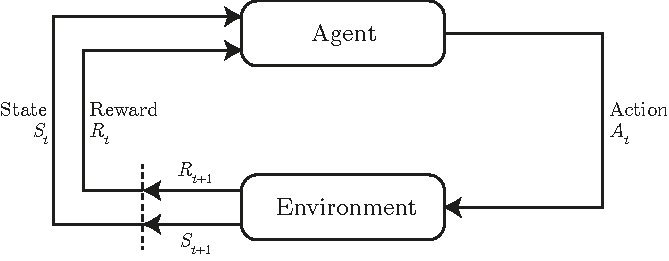
\includegraphics[scale=1]{../include/agent-environment-loop.pdf}
    \caption{The Agent-Environment interface adapted from \citet[chap. 3]{RLBook2018}}
    \label{fig:agent-environment}
\end{figure}

As such, the agent will learn the optimal \textit{policy} $\pi^*$ (or estimate thereof) by iteratively taking actions, and observing the following reward, and state of the environment.

To give a small example of the Markov decision process, consider the small grid world in \cref{fig:gridworld}. 
Suppose a robot is initially placed in square $a$, labeled \texttt{Start}, and that it has the goal of navigating to square $d$, labeled \texttt{End}. 
If the robot moves off the grid, it is returned to square $a$. 
Every move the robot makes have a cost of one, except for when successfully navigating to the \texttt{End} square, in which case it is rewarded with one point. 
Finally, suppose that the robot is faulty, and whenever it attempts to go right, there is a 20\% probability of moving diagonally down-right.
An MDP describing this problem is visualized in \cref{fig:gridworldMDP}.

\begin{figure}[!htb]
    \centering
    \begin{minipage}[t]{0.34\textwidth}
        \centering
        \raisebox{-0.5\height}{\hbox{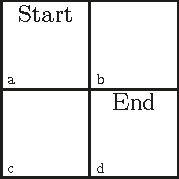
\includegraphics{../include/PDF/gridworld2x2.pdf}}}
        \subcaption{2x2 gridworld}
        \label{fig:gridworld}
    \end{minipage}
    \begin{minipage}[t]{0.6\textwidth}
        \centering
        \raisebox{-0.5\height}{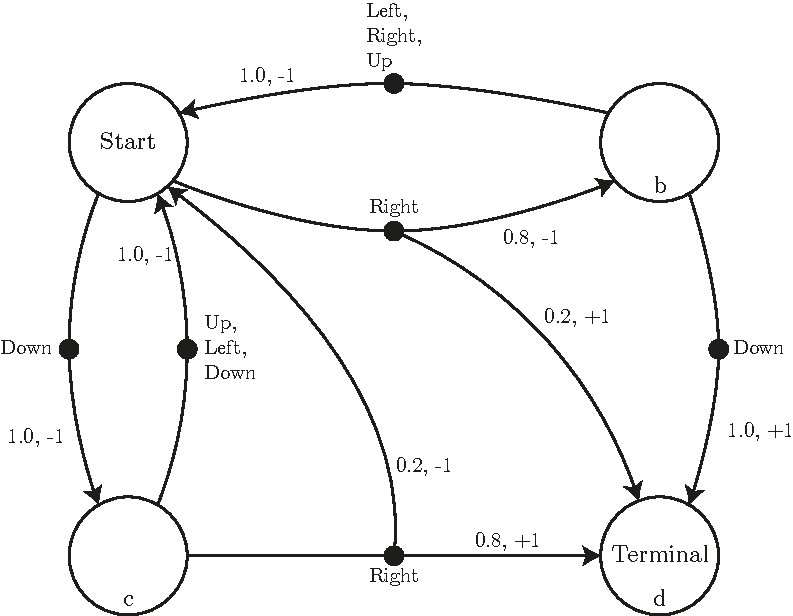
\includegraphics[scale=0.6]{../include/PDF/MDP.pdf}}
        \subcaption{MDP visualization of example gridworld with error prone right move}
        \label{fig:gridworldMDP}
    \end{minipage}
    \caption{Example environment (a) and MDP describing it (b)}
    \label{fig:MDP}
\end{figure}



\subsection{RL}



\subsubsection{Model-based \& Model-free}

\subsubsection{On-policy \& Off-policy}

\subsubsection{Reinforcement learning algorithm classes}
\paragraph{Action-Value}
\paragraph{Policy-Gradient}
\paragraph{Actor-Critic}

\subsubsection{Exploration vs Exploitation}
A great dilemma in the field of reinforcement learning is the choice of exploration vs. exploitation, when should the agent perform the action it deems best according to previous experience, and when should it explore new actions of which the outcome is less known? 
The most straightforward action-selection approach would be greedy action selection. With a greedy action selection, initial action values are essential, as otherwise, the agent may never explore some actions --- if there is an action which the agent has not yet attempted, it must see that action as attractive to get some idea of the usefulness of every action. 

An improvement to the greedy action selection, which has performed well historically is the $\epsilon-greedy$ approach, where the agent picks a random action with probability $\epsilon$, and a greedy action with probability $1-\epsilon$.

\begin{align}
    \Pr{A_t = a \in_R \mycal{A}(S_t)} &= \epsilon\\
    \Pr{A_t = \argmax_a \left[Q_t(S_t,a)\right]} &= 1-\epsilon
\end{align}

Where $Q_t$ is the action-value function estimate at time $t$.


% ------------------------------
\clearpage
\label{Bibliography}
\lhead{\emph{Bibliography}}
\rhead{}
\replace{TODO: standardize references}
\bibliography{bib/Bibliography}
\nocite{*}


%%%%%%%%%%%%%%
% Appendices
%%%%%%%%%%%%%%
\clearpage
\label{Appendix}
\addtocontents{toc}{\vspace{2em}}
\appendix
\lhead{\emph{Appendix A}}
\section{Technical drawings}
\label{appendix:techdraw}
\begin{figure}[!htb]
    \centering
    \includeinkscape[scale=3]{signaturer}
    \caption{Induction loop drawing legend}
    \label{fig:inductionsignatures}
\end{figure}
\begin{table}[!htb]
    \centering
    \begin{tabular}{|l|l|}\hline
        Regular Expression & Explanation \\\hline
        {[A-B]}[1-2] & Group of upstream movements on single road\\\hline
        \textcolor{gray}{[A-B][1-2]}Cy & Bicycle movement modifier\\\hline
        \textcolor{gray}{[A-B][1-2]}[Vv] & Left-turn modifier\\\hline
        \textcolor{gray}{[A-B][1-2]}[Hh] & Right-turn modifier\\\hline
        [A-B][1-2](Cy)?([Hh] | [Vv])? & Non-pedestrian movement strings\\\hline
        [a-b][f-g] & Pedestrian light\\\hline
    \end{tabular}
    \caption{Explanation of traffic movement strings used in later drawing. Occasionally the movements seem aggregated in the drawing, e.g. B1+B1h; this does not mean that they follow the same light, but rather that multiple lights share the same approximate physical location.}
    \label{tab:intersectionmovements}
\end{table}
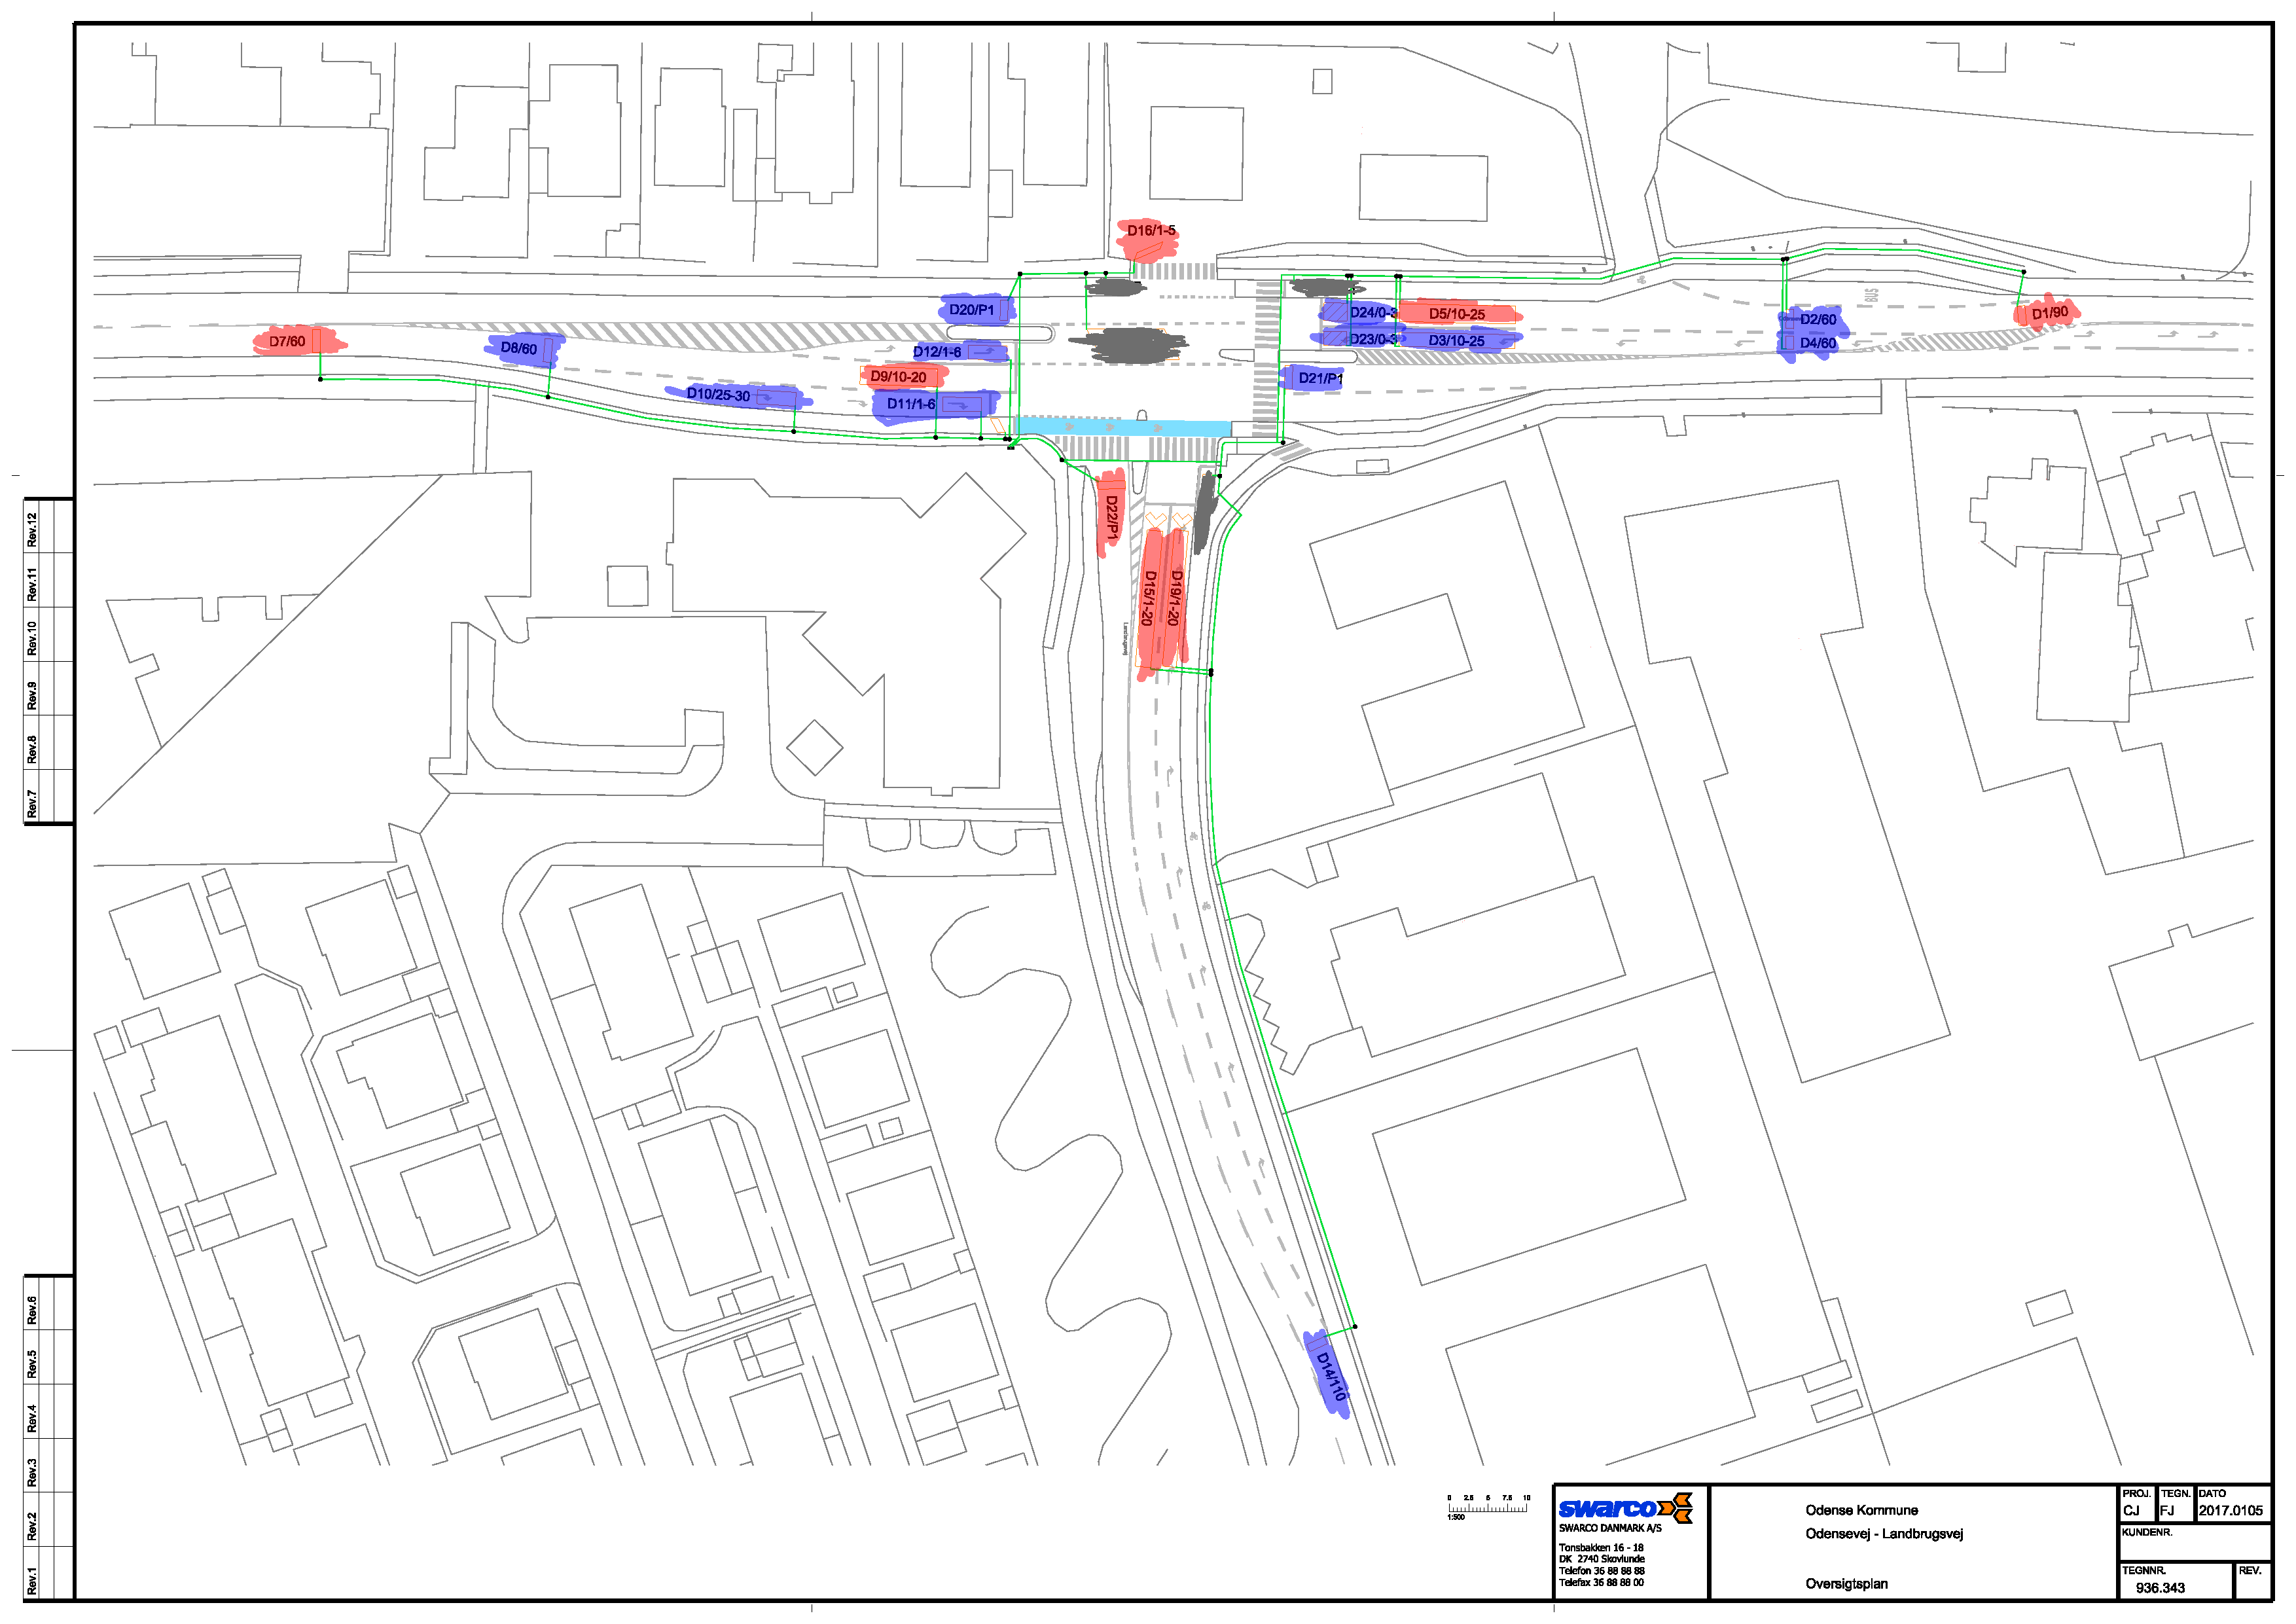
\includepdf[angle=270]{../include/Anl-427-induction-loop.pdf}
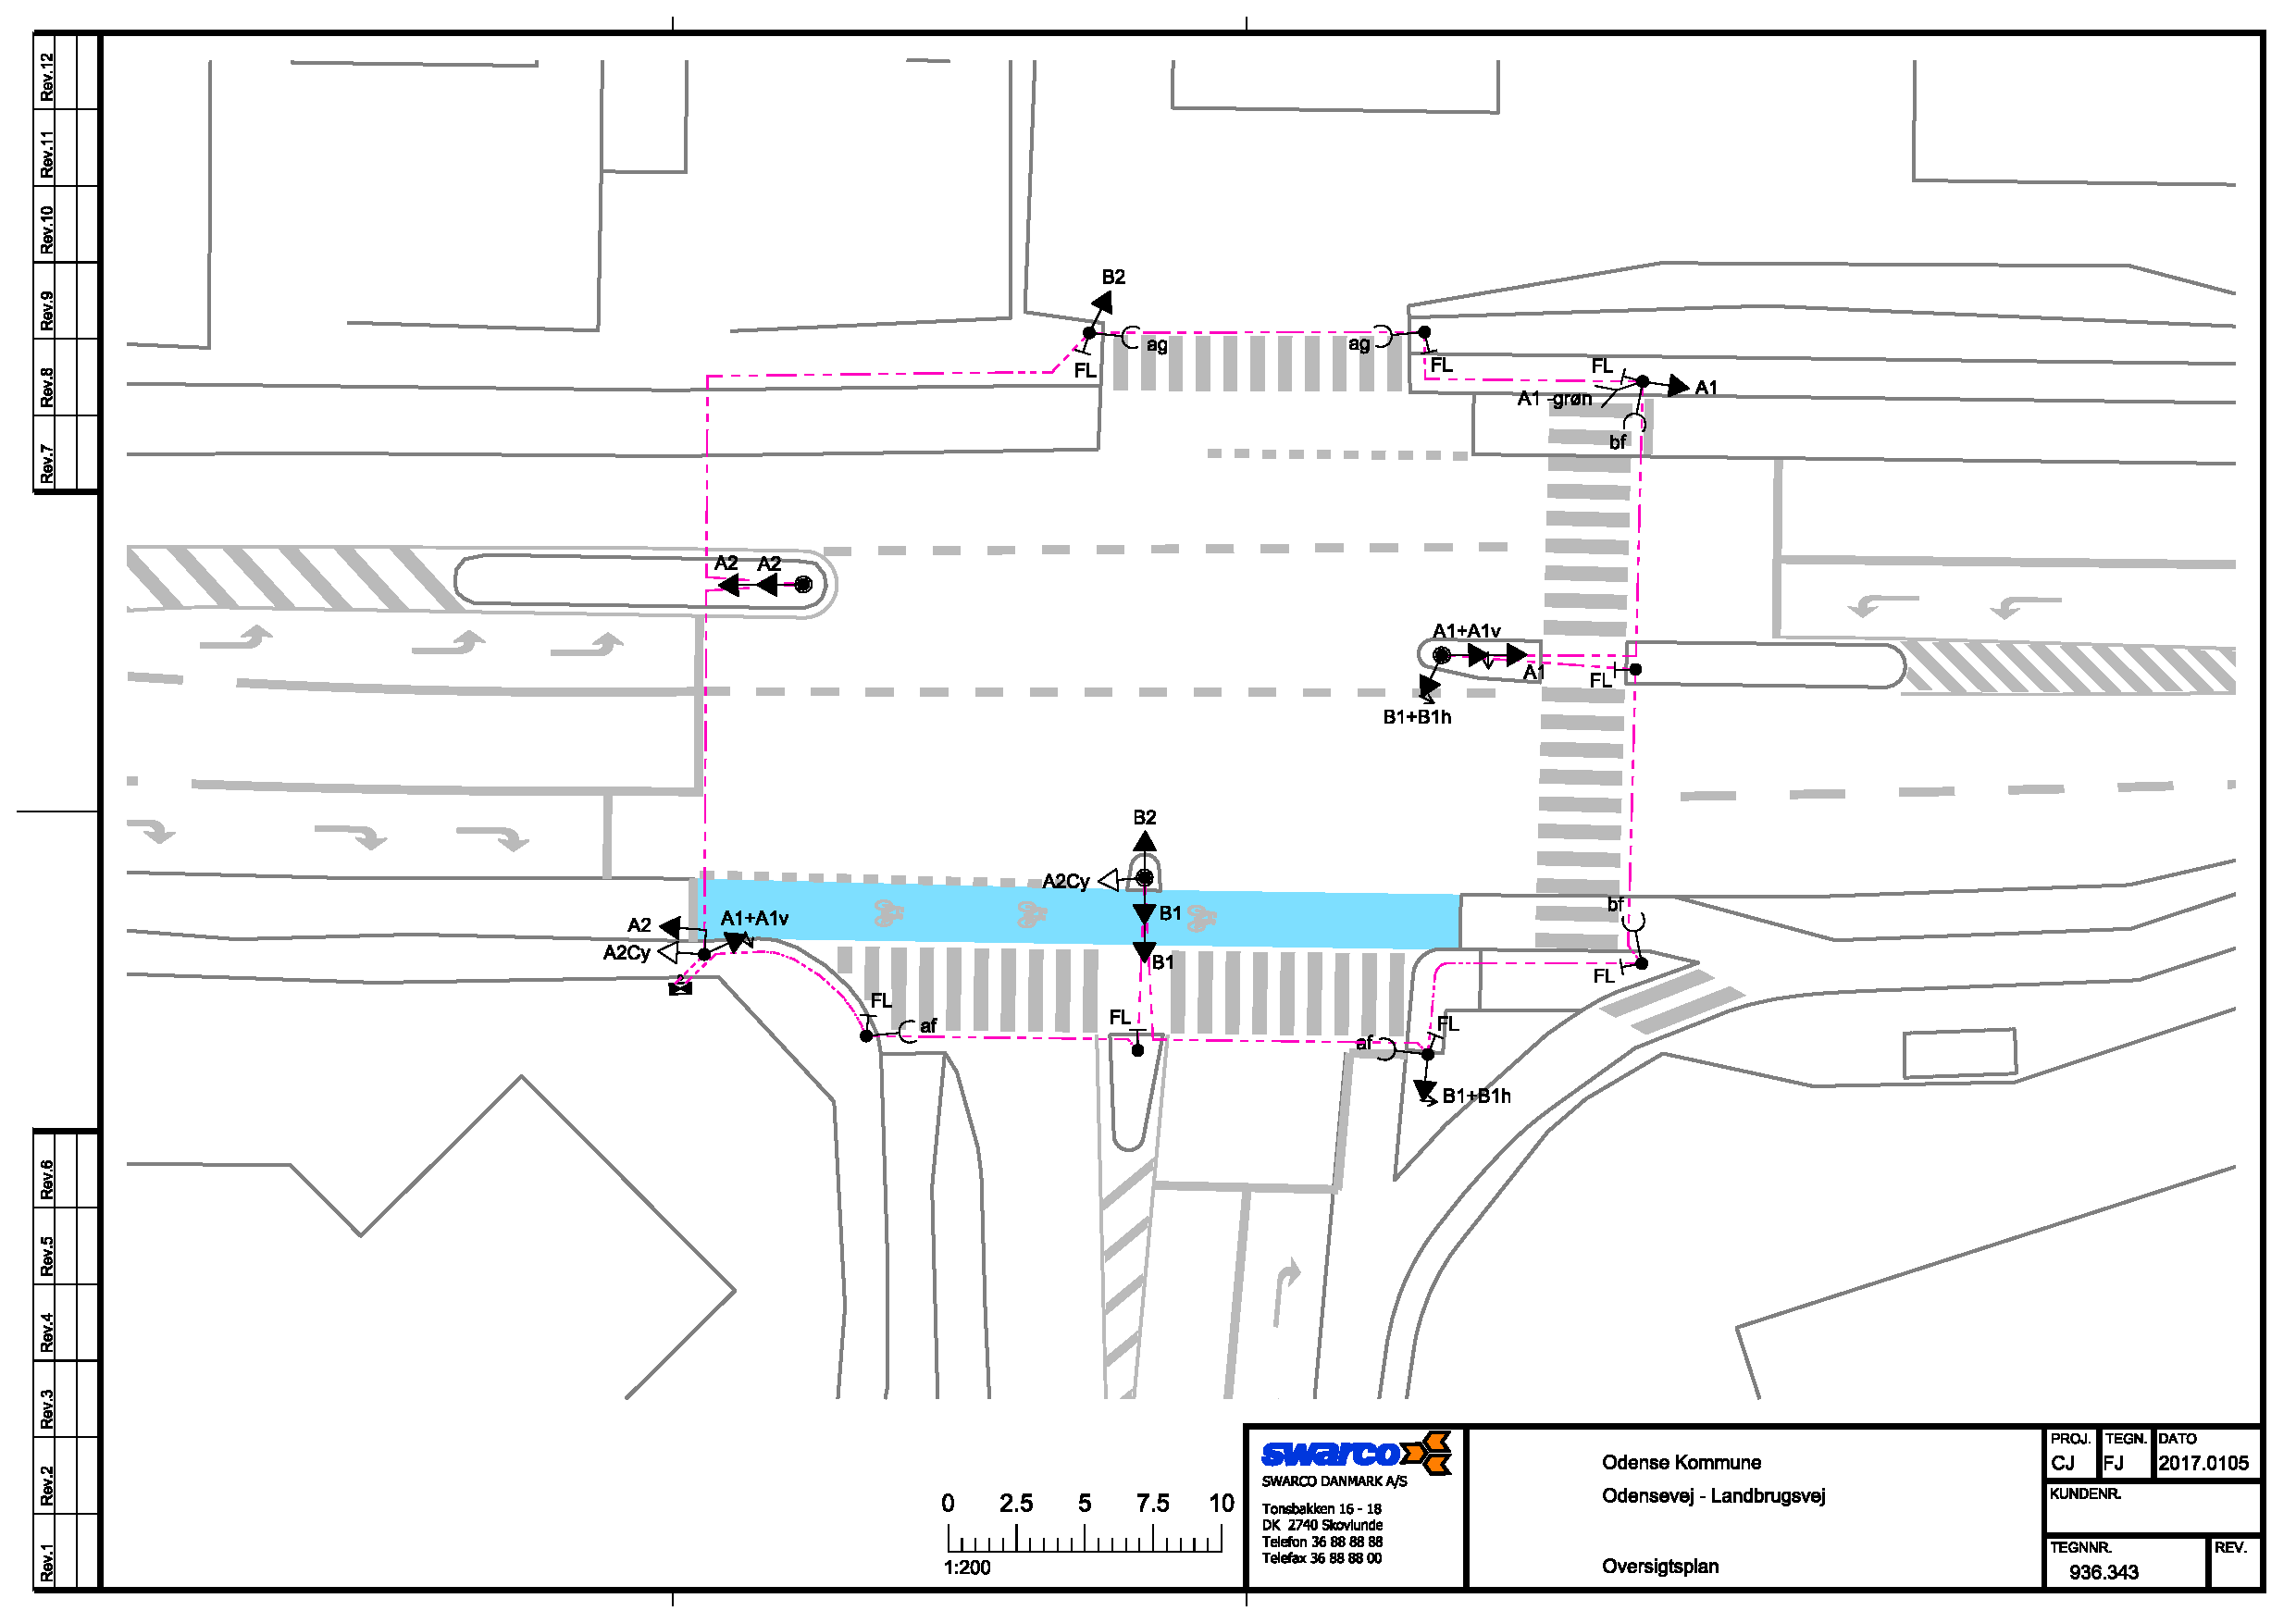
\includepdf[angle=270]{../include/Anl-427-traffic-light-movement.pdf}
\addtocontents{toc}{\vspace{2em}}





\end{document}
